No primeiro teste, foi medido o tempo gasto com a gera��o de terrenos. Para cada n�mero de \emph{octaves} (4, 16 e 32), foi gerado 100 terrenos, e medido o tempo gasto.

Nas Tabelas \ref{tabela:geracao1} e \ref{tabela:geracao2} � apresentado os tempos das chamadas �s fun��es respons�veis pela gera��o dos terrenos, considerando o algoritmo de ru�do de Perlin. Abaixo uma explica��o sobre cada fun��o:

\begin{itemize}
	\item {\bf FillHeightmap}: Constr�i o terreno, determinando a altura e posi��o de cada v�rtice e armazena em um vetor de \emph{float}. Sua complexidade de tempo � proporcional � largura do terreno (\emph{n}), ao comprimento (\emph{m}) e ao n�mero de \emph{octaves} (\emph{c}). \emph{O(n*m*c)}.
	\item {\bf CopyHeightmap}: Copia o vetor, constru�do na fun��o \emph{FillHeightmap} para um novo vetor VBO. Sua complexidade de tempo � proporcional � largura do terreno (\emph{n}) e ao comprimento (\emph{m}). \emph{O(n*m)}.
	\item {\bf BuildVBOs}: Modifica os ponteiros para o desenho dos vetores VBO. � independente do tamanho do vetor.
\end{itemize}

\begin{table}[H]
	\begin{center}
		\begin{tabular}{|c|c|c|c|c|c|c|}
			\hline
			 - & \multicolumn{3}{|c|}{FillHeightMap} & \multicolumn{3}{|c|}{CopyHeightMap} \\
			\hline
			\emph{Octaves} & \scriptsize M�n. & \scriptsize M�x. & \scriptsize M�dia & \scriptsize M�n. & \scriptsize M�x. & \scriptsize M�dia \\
			\hline
			4 & 0,0410248 & 0,0536568 & 0,0443777 & 0,0737747 & 0,0866761 & 0,0782942 \\
			\hline
			16 & 0,1644840 & 0,2593410 & 0,1698030 & 0,0710867 & 0,0865546 & 0,0734247 \\
			\hline
			32 & 0,3315010 & 0,4503400 & 0,3405685 & 0,0708154 & 0,0778093 & 0,0730120 \\
			\hline
			
		\end{tabular}
		\caption{Tempos da gera��o dos terrenos (em segundos)}
		\label{tabela:geracao1}
	\end{center}
\end{table}

\begin{table}[H]
	\begin{center}
		\begin{tabular}{|c|c|c|c|c|c|c|}
			\hline
			 - & \multicolumn{3}{|c|}{BuildVBOs} & \multicolumn{3}{|c|}{Total}  \\
			\hline
			\emph{Octaves} & \scriptsize M�n. & \scriptsize M�x. & \scriptsize M�dia & \scriptsize M�n. & \scriptsize M�x. & \scriptsize M�dia \\
			\hline
			4 & 0,0078359 & 0,0161562 & 0,0107964 & 0,1264320 & 0,1498800 & 0,1336476 \\
			\hline
			16 & 0,0081773 & 0,0407795 & 0,0114127 & 0,2469740 & 0,3459500 & 0,2550180 \\
			\hline
			32 & 0,0075448 & 0,0129804 & 0,0093645 & 0,4121210 & 0,5310980 & 0,4231183 \\
			\hline
		\end{tabular}
		\caption{Tempos da gera��o dos terrenos (em segundos)}
		\label{tabela:geracao2}
	\end{center}
\end{table}



A Tabela \ref{tabela:geracao3} apresenta os percentuais de tempo de cada chamada da fun��o em rela��o ao tempo m�dio total gasto com a gera��o de um terreno. A Figura \ref{fig:geracao3} mostra um gr�fico com esses dados.

\begin{table}[H]
	\begin{center}
		\begin{tabular}{|c|c|c|c|c|}
			\hline
			\emph{Octaves} & FillHeightMap & CopyHeightMap & BuildVBOs & Total  \\
			\hline
			4 & 32,2\% & 58,6\% & 9,2\% & 100\% \\
			\hline
			16 & 66,6\% & 28,8\% & 4,6\% & 100\% \\
			\hline
			32 & 80,5\% & 17,3\% & 2,2\% & 100\% \\
			\hline
		\end{tabular}
		\caption{Porcentagem dos tempos m�dios de cada chamada, com n�mero vari�vel de \emph{octaves}}
		\label{tabela:geracao3}
	\end{center}
\end{table}


\begin{figure}[H]
	\center{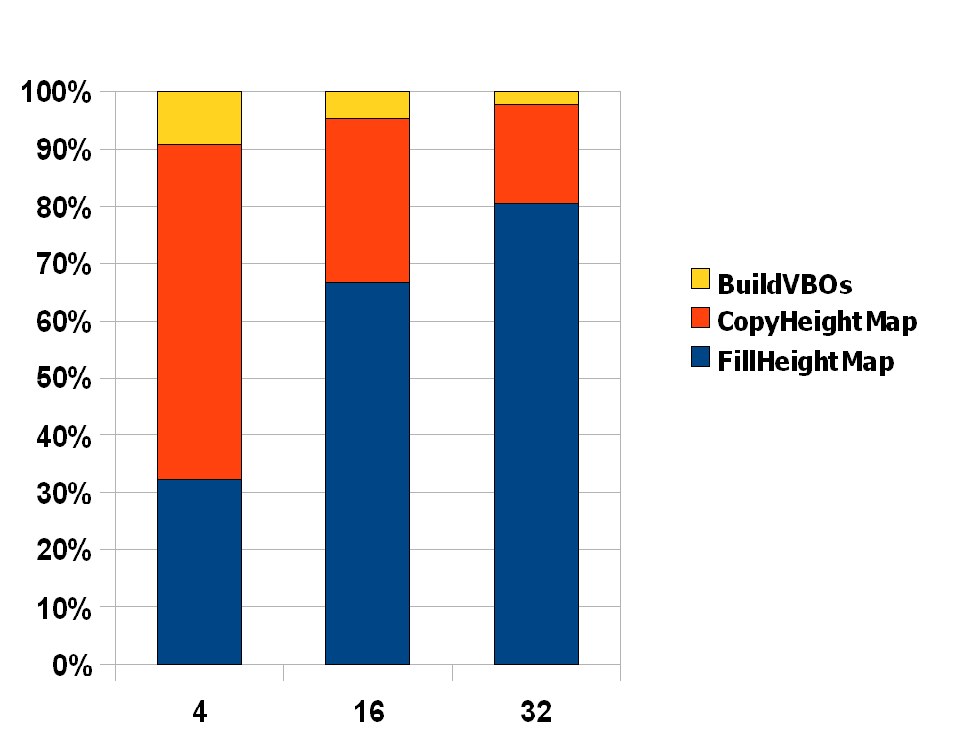
\includegraphics[width=0.5\linewidth]{testes/testes.png}}
	\caption{\label{fig:geracao3} Gr�fico com a porcentagem dos tempos m�dios de cada chamada, com n�mero vari�vel de \emph{octaves}}
\end{figure}

Como podemos observar, o tempo gasto com a c�pia dos dados para a nova estrutura de dados ({\bf CopyHeightMap}) gasta um tempo consider�vel nas tr�s medi��es (com 4, 16 e 32 octaves), algo a ser considerado em trabalhos futuros.